\subsection{UC37: Gestione credenziali}
\label{sec:UC37}
\begin{figure}[!ht]
    \caption{Diagramma di UC37: Gestione credenziali}
    \vspace{10px}
    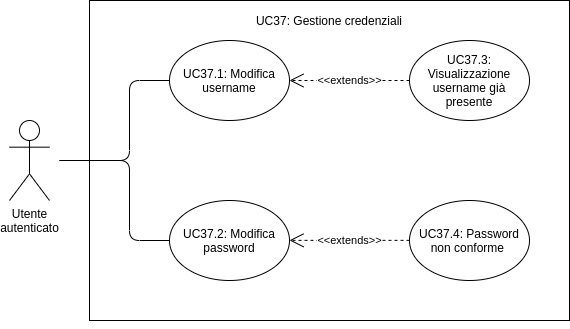
\includegraphics[scale=0.5]{../../../Images/AnalisiRequisiti/UC37}
    \centering
\end{figure}

\begin{itemize}
    \item \textbf{Descrizione:} l'utente vuole gestire le proprie credenziali;
    \item \textbf{Attore Primario:} utente autenticato;
    \item \textbf{Attore Secondario:} servizio di autenticazione esterno;
    \item \textbf{Precondizione:} l'utente si trova all'interno del proprio profilo;
    \item \textbf{Postcondizione:} l'utente può modificare le proprie credenziali;
    \item \textbf{Scenario Principale:}
          \begin{itemize}
              \item  l'utente decide cosa modificare tra:
                    \begin{itemize}
                        \item username \underline{\hyperref[sec:UC37.1]{UC37.1}};
                        \item password  \underline{\hyperref[sec:UC37.2]{UC37.2}}.
                    \end{itemize}
          \end{itemize}
\end{itemize}

\subsubsection{UC37.1 Modifica dell'username}
\label{sec:UC37.1}
\begin{itemize}
    \item \textbf{Descrizione:} l'utente vuole modificare il proprio username;
    \item \textbf{Attore Primario:} utente autenticato;
    \item \textbf{Attore Secondario:} servizio di autenticazione esterno;
    \item \textbf{Precondizione:} l'utente si trova all'interno del proprio profilo;
    \item \textbf{Postcondizione:} l'utente può modificare il proprio username;
    \item \textbf{Estensione:} visualizzazione errore se lo username è già presente nel database \underline{\hyperref[sec:UC37.3]{UC37.3}}.
\end{itemize}

\subsubsection{UC37.2 Modifica della password}
\label{sec:UC37.2}
\begin{itemize}
    \item \textbf{Descrizione:} l'utente vuole modificare la propria password;
    \item \textbf{Attore Primario:} utente autenticato;
    \item \textbf{Attore Secondario:} servizio di autenticazione esterno;
    \item \textbf{Precondizione:} l'utente si trova all'interno del proprio profilo;
    \item \textbf{Postcondizione:} l'utente può modificare la propria password.
    \item \textbf{Estensione:} La password inserita non è conforme ai requisiti:
          \begin{itemize}
              \item L'utente può reinserire la password rispettando i requisiti.
          \end{itemize}
\end{itemize}
\subsubsection{UC37.3: Visualizzazione username già presente}
\label{sec:UC37.3}
\begin{itemize}
    \item \textbf{Descrizione:} Visualizzazione di un errore se lo username è già in uso;
    \item \textbf{Attore Primario:} utente autenticato;
    \item \textbf{Attore Secondario:} servizio di autenticazione esterno;
    \item \textbf{Precondizione:} l'utente ha inserito uno username non disponibile perché già usato;
    \item \textbf{Postcondizione:} l'utente visualizza un messaggio di errore.
\end{itemize}

\subsubsection{UC37.4: Password non conforme}
\label{sec:UC37.4}
\begin{itemize}
    \item \textbf{Descrizione:} Visualizzazione di un errore se la password non è conforme ai requisiti;
    \item \textbf{Attore Primario:} utente autenticato;
    \item \textbf{Attore Secondario:} Amazon Cognito;
    \item \textbf{Precondizione:} l'utente ha inserito una password non conforme ai requisiti, che sono:
          \begin{itemize}
              \item lunghezza almeno di 8 caratteri;
              \item contenga almeno una lettera maiuscola;
              \item contenga almeno una lettera minuscola;
              \item contenga almeno un numero;
              \item contenga almeno un carattere speciale.
          \end{itemize}
    \item \textbf{Postcondizione:} l'utente visualizza un messaggio di errore.
\end{itemize}